\documentclass{article}
\usepackage{draftwatermark}
\usepackage{longtable}
\SetWatermarkText{DRAFT}
\SetWatermarkScale{1}

\author{Michael Edwards\\ 
  James Woods}
\title{Housing Market Institutions Drive Race and Ethnicity Differences in Energy Consumption}


\usepackage{Sweave}
\begin{document}
\maketitle
\Sconcordance{concordance:DraftEdwardsWoods.tex:DraftEdwardsWoods.Rnw:%
1 10 1 1 0 12 1 1 310 1 7 6 1 1 3 16 0 1 2 4 1 1 3 1 2 8 1 1 3 1 2 13 1 %
1 8 62 0 1 3 4 1 1 15 100 0 1 2 2 1 1 7 46 0 1 3 1 1 1 6 16 0 1 1 223 0 %
1 3 4 1 1 50 10 1}


\begin{abstract}

When socio-demographic factors are considered in any kind of analysis of household electric and gas utility data, it is common to observe differences in energy use between households with different self-reported race and ethnicity compositions. These differences persist controlling for structure type, e.g., single family dwelling, age and size of housing units, and, other common control variables. Without the information necessary to better explain these differences, they are commonly summarized simply as cultural differences. This paper demonstrates that these differences can be partially explained by differential sorting by structure and ownership, i.e., endogenizing housing choice and rental decisions. We will show that these differences in energy consumption may be because of housing market institutions and restrictions.
\end{abstract}

\section{Introduction}


\begin{itemize}

  \item Differences in energy use by race and ethnicity is frequently reported in the literature
  \item Much of the difference has to do with differences in income levels and education but not frequently modeled correctly.
  \item Even with proper race and ethnicity controls with income, some patterns persist.
  \item We assert that these differences are caused, at least in part, by housing discrimination, forcing people into housing types different than what they would prefer without discrimination; and renting rather than buying.
  \item We show this with a model that endogenizes structure type and tenure decision.
  \item emphasize that this is early work.
\end{itemize}

%\cite{RBase}




  \subsection{Race and Ethnicity in Conditional Demand}
  
  \subsection{How Race and Ethnicity are Interpreted}

\section{RECS}

\begin{itemize}
  \item Description on RECS data size number of observations sampling method etc.
  \item Scope of data  
  \item Weighting to account for stratified sampling
  \item We need more tables and graphics here.
\end{itemize}



% latex table generated in R 3.0.1 by xtable 1.7-4 package
% Fri Mar 27 15:58:26 2015
\begin{table}[ht]
\centering
\begin{tabular}{rrrrrr}
  \hline
 & Mobile & SFDetached & SFAttached & SmApartment & LgApartment \\ 
  \hline
FALSEWt & 371 & 5694 & 544 & 430 & 951 \\ 
  FALSEAfAm &  24 & 754 & 121 & 174 & 382 \\ 
  FALSEAsian &   1 & 231 &  48 &  52 & 113 \\ 
  FALSEMulti &   6 &  87 &  14 &  12 &  27 \\ 
  FALSENativeAm &   7 &  35 &   9 &   7 &  15 \\ 
  FALSEOther &   2 &  59 &   8 &  13 &  29 \\ 
  FALSEPacific &   1 &  22 &   1 &   2 &  10 \\ 
  TRUEAfAm &   3 &   8 &  10 &   5 &   8 \\ 
  TRUEAsian &   0 &   5 &   0 &   0 &   1 \\ 
  TRUEMulti &   1 &  10 &   2 &   4 &   4 \\ 
  TRUENativeAm &   2 &  17 &   3 &   6 &   9 \\ 
  TRUEOther &   6 &  41 &  12 &  16 &  24 \\ 
  TRUEPacific &   0 &   2 &   1 &   1 &   0 \\ 
  TRUEWt &  97 & 730 & 105 & 184 & 332 \\ 
   \hline
\end{tabular}
\caption{Count of Observations by Race and Structure Type} 
\label{tab:RaceVStruct}
\end{table}
% latex table generated in R 3.0.1 by xtable 1.7-4 package
% Fri Mar 27 15:58:26 2015
\begin{table}[ht]
\centering
\begin{tabular}{rrrrrr}
  \hline
 & Mobile & SFDetached & SFAttached & SmApartment & LgApartment \\ 
  \hline
NE &  47 & 1173 & 218 & 326 & 470 \\ 
  MidWest &  92 & 2080 & 162 & 145 & 323 \\ 
  South & 245 & 2685 & 257 & 226 & 603 \\ 
  West & 137 & 1757 & 241 & 209 & 509 \\ 
   \hline
\end{tabular}
\caption{Count of Observations by Region and Structure Type} 
\label{tab:RegionVStruct}
\end{table}
\begin{figure}
\begin{center}
\caption{Annual kWh by Rent/Own and Race}
\label{fig:kWhbyOwnRace}
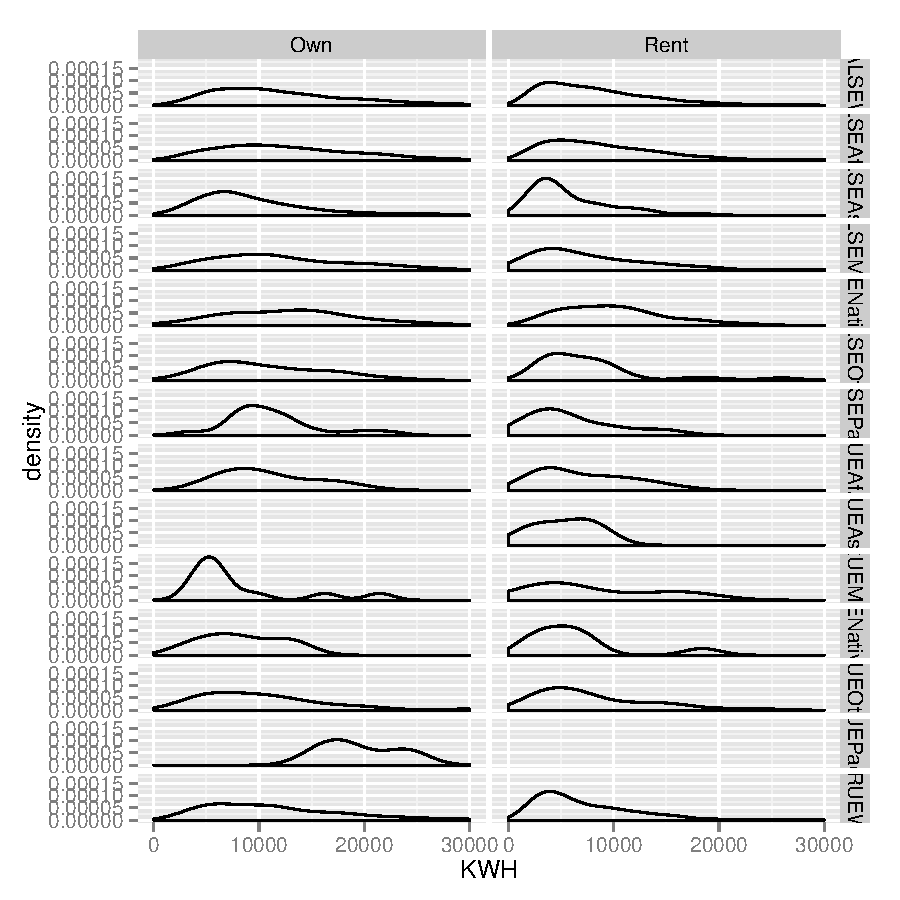
\includegraphics{DraftEdwardsWoods-005}
\end{center}
\end{figure}



\begin{figure}
\begin{center}
\caption{Annual kWh by Income}
\label{fig:kWhbyIncome}
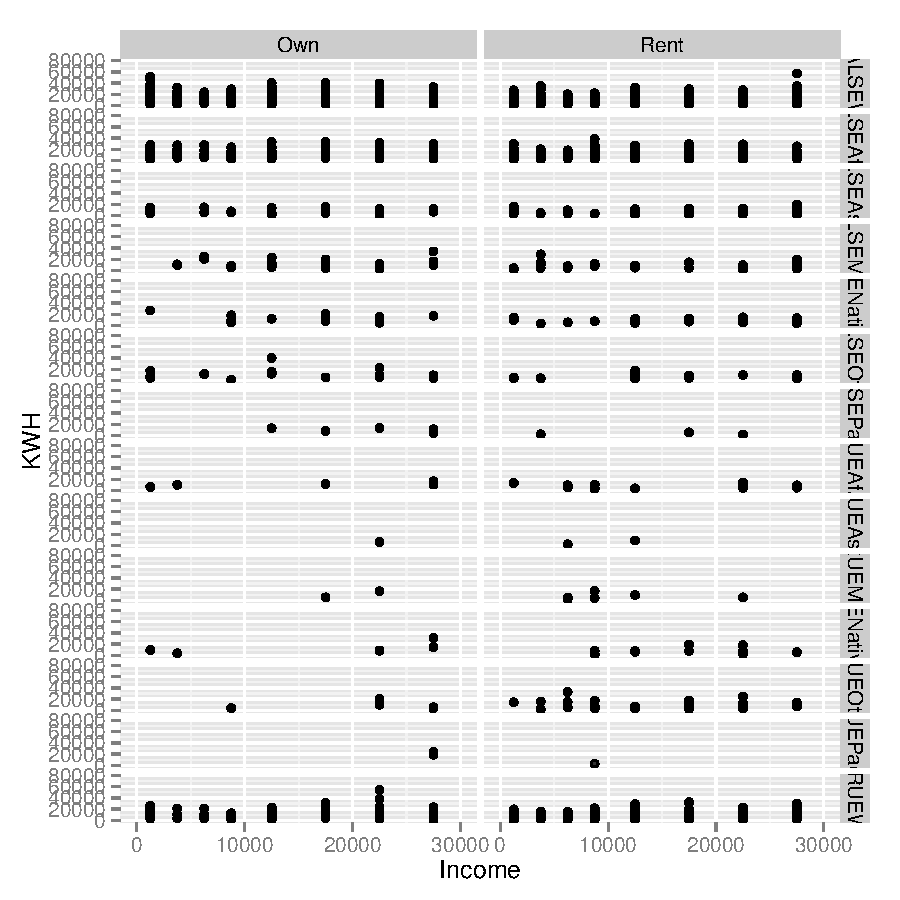
\includegraphics{DraftEdwardsWoods-006}
\end{center}
\end{figure}

\begin{figure}
\begin{center}\label{fig:HHbyRace}
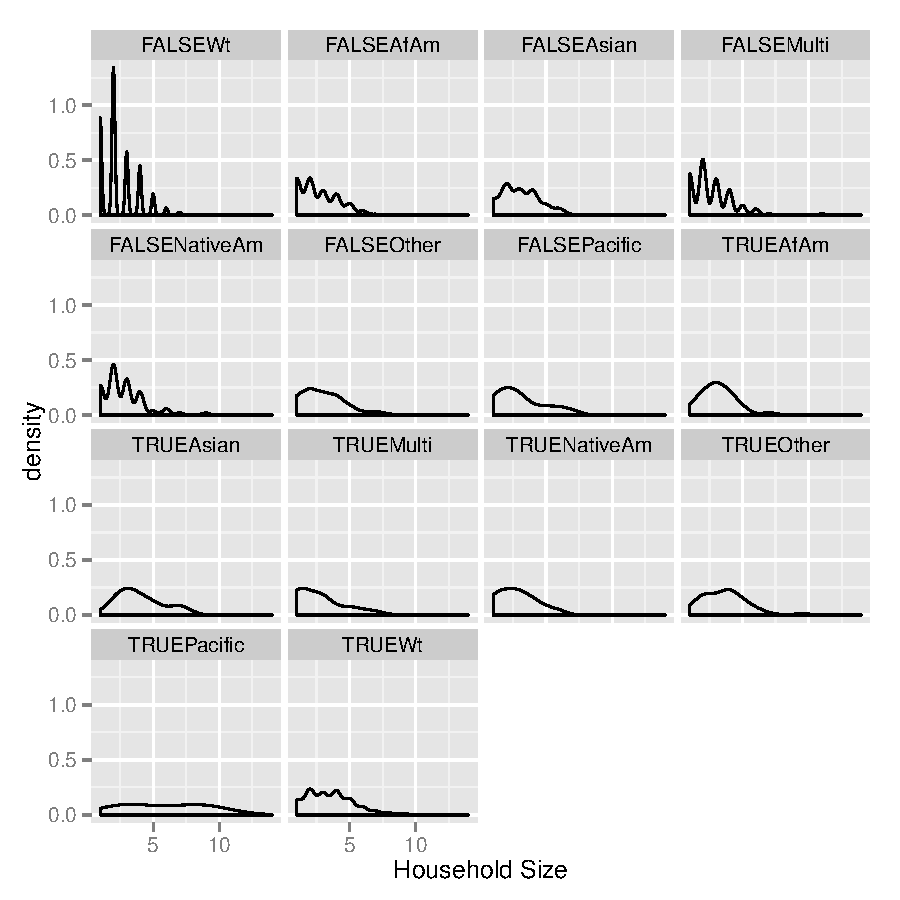
\includegraphics{DraftEdwardsWoods-007}
\end{center}
\end{figure}


  \subsection{Race and Ethnicity Differences in Equipment and Structure}

\begin{itemize}
  \item differences in structure type x
  \item difference in tenure x
  \item differences in energy star controlling for own rent
  \item general differences in own vs rent.  
  \item explain with split incentives story
  \item difference in age of structure x
  \item differences in hot water fuel x
  \item difference in heating fuel x
    \item difference in climate/location x
\end{itemize}
  
  


  
% latex table generated in R 3.0.1 by xtable 1.7-4 package
% Fri Mar 27 15:58:43 2015
\begin{table}[ht]
\centering
\begin{tabular}{rrr}
  \hline
 & FALSE & TRUE \\ 
  \hline
FALSEWt & 7606 & 384 \\ 
  FALSEAfAm & 1367 &  88 \\ 
  FALSEAsian & 424 &  21 \\ 
  FALSEMulti & 133 &  13 \\ 
  FALSENativeAm &  68 &   5 \\ 
  FALSEOther & 102 &   9 \\ 
  FALSEPacific &  30 &   6 \\ 
  TRUEAfAm &  31 &   3 \\ 
  TRUEAsian &   4 &   2 \\ 
  TRUEMulti &  19 &   2 \\ 
  TRUENativeAm &  36 &   1 \\ 
  TRUEOther &  88 &  11 \\ 
  TRUEPacific &   4 &   0 \\ 
  TRUEWt & 1330 & 118 \\ 
   \hline
\end{tabular}
\caption{EnergyStar Wall AC by Race and Ethnicity} 
\label{tab:EnergyStarWall}
\end{table}

% latex table generated in R 3.0.1 by xtable 1.7-4 package
% Fri Mar 27 15:58:43 2015
\begin{table}[ht]
\centering
\begin{tabular}{rrr}
  \hline
 & Rural & Urban \\ 
  \hline
FALSEWt & 1937 & 6053 \\ 
  FALSEAfAm & 192 & 1263 \\ 
  FALSEAsian &  14 & 431 \\ 
  FALSEMulti &  28 & 118 \\ 
  FALSENativeAm &  25 &  48 \\ 
  FALSEOther &  12 &  99 \\ 
  FALSEPacific &   4 &  32 \\ 
  TRUEAfAm &   6 &  28 \\ 
  TRUEAsian &   0 &   6 \\ 
  TRUEMulti &   1 &  20 \\ 
  TRUENativeAm &   3 &  34 \\ 
  TRUEOther &   5 &  94 \\ 
  TRUEPacific &   2 &   2 \\ 
  TRUEWt & 137 & 1311 \\ 
   \hline
\end{tabular}
\caption{Race by Urban/Rural} 
\label{tab:UrbRural}
\end{table}

% latex table generated in R 3.0.1 by xtable 1.7-4 package
% Fri Mar 27 15:58:43 2015
\begin{table}[ht]
\centering
\begin{tabular}{rrrrrrrrr}
  \hline
 & NG & LPG & Oil & Kerosene & Elec & Wood & Solar & Other \\ 
  \hline
FALSEWt & 4077 & 315 & 361 &   3 & 3190 &  11 &  12 &   7 \\ 
  FALSEAfAm & 755 &  17 &  35 &   0 & 640 &   0 &   2 &   0 \\ 
  FALSEAsian & 312 &   7 &  12 &   0 & 109 &   0 &   0 &   2 \\ 
  FALSEMulti &  85 &   5 &   3 &   0 &  53 &   0 &   0 &   0 \\ 
  FALSENativeAm &  34 &   2 &   1 &   0 &  36 &   0 &   0 &   0 \\ 
  FALSEOther &  57 &   3 &   6 &   0 &  44 &   0 &   0 &   0 \\ 
  FALSEPacific &  15 &   0 &   2 &   0 &  17 &   0 &   2 &   0 \\ 
  TRUEAfAm &  20 &   0 &   1 &   0 &  13 &   0 &   0 &   0 \\ 
  TRUEAsian &   5 &   0 &   0 &   0 &   1 &   0 &   0 &   0 \\ 
  TRUEMulti &  12 &   0 &   1 &   0 &   8 &   0 &   0 &   0 \\ 
  TRUENativeAm &  29 &   0 &   0 &   0 &   8 &   0 &   0 &   0 \\ 
  TRUEOther &  62 &   1 &   5 &   0 &  30 &   0 &   0 &   0 \\ 
  TRUEPacific &   1 &   1 &   0 &   0 &   2 &   0 &   0 &   0 \\ 
  TRUEWt & 830 &  33 &  26 &   0 & 552 &   0 &   1 &   0 \\ 
   \hline
\end{tabular}
\caption{Water Service by Race and Ethnicity} 
\label{tab:Water}
\end{table}
% latex table generated in R 3.0.1 by xtable 1.7-4 package
% Fri Mar 27 15:58:43 2015
\begin{table}[ht]
\centering
\begin{tabular}{rrrrrrrrrr}
  \hline
 & NG & LPG & Oil & Kerosene & Elec & Wood & Solar & District & Other \\ 
  \hline
FALSEWt & 3987 & 400 & 642 &  40 & 2515 & 245 &   1 &  11 &  19 \\ 
  FALSEAfAm & 674 &  29 &  60 &   6 & 640 &  10 &   0 &   5 &   0 \\ 
  FALSEAsian & 249 &   1 &  21 &   0 & 122 &   1 &   0 &   2 &   0 \\ 
  FALSEMulti &  80 &   6 &   7 &   0 &  41 &   7 &   0 &   0 &   1 \\ 
  FALSENativeAm &  34 &   3 &   1 &   0 &  33 &   2 &   0 &   0 &   0 \\ 
  FALSEOther &  59 &   1 &   9 &   0 &  36 &   3 &   0 &   0 &   0 \\ 
  FALSEPacific &  16 &   0 &   2 &   0 &   5 &   1 &   0 &   0 &   0 \\ 
  TRUEAfAm &  21 &   0 &   1 &   1 &   9 &   0 &   0 &   0 &   0 \\ 
  TRUEAsian &   4 &   0 &   0 &   0 &   1 &   0 &   0 &   0 &   0 \\ 
  TRUEMulti &  11 &   0 &   4 &   0 &   4 &   1 &   0 &   0 &   0 \\ 
  TRUENativeAm &  26 &   1 &   2 &   0 &   7 &   0 &   0 &   0 &   0 \\ 
  TRUEOther &  53 &   0 &   8 &   1 &  32 &   0 &   0 &   2 &   0 \\ 
  TRUEPacific &   1 &   0 &   0 &   0 &   2 &   0 &   0 &   0 &   0 \\ 
  TRUEWt & 604 &  25 &  51 &   2 & 540 &  18 &   0 &   3 &   1 \\ 
   \hline
\end{tabular}
\caption{Heating Fuel by Race and Ethnicity} 
\label{tab:HeatFuel}
\end{table}
% latex table generated in R 3.0.1 by xtable 1.7-4 package
% Fri Mar 27 15:58:43 2015
\begin{table}[ht]
\centering
\begin{tabular}{rrrrrr}
  \hline
 & VColdCold & HotDryMixedDry & HotHumid & MixedHumid & Marine \\ 
  \hline
FALSEWt & 3118 & 850 & 1216 & 2382 & 424 \\ 
  FALSEAfAm & 299 & 131 & 383 & 611 &  31 \\ 
  FALSEAsian &  95 & 128 &  60 &  77 &  85 \\ 
  FALSEMulti &  51 &  27 &  13 &  40 &  15 \\ 
  FALSENativeAm &  23 &  10 &   7 &  28 &   5 \\ 
  FALSEOther &  29 &  16 &  24 &  37 &   5 \\ 
  FALSEPacific &   4 &   6 &  13 &   4 &   9 \\ 
  TRUEAfAm &  16 &   5 &   4 &   9 &   0 \\ 
  TRUEAsian &   2 &   2 &   1 &   0 &   1 \\ 
  TRUEMulti &  12 &   6 &   1 &   0 &   2 \\ 
  TRUENativeAm &   9 &  14 &   1 &   8 &   5 \\ 
  TRUEOther &  35 &  19 &  10 &  28 &   7 \\ 
  TRUEPacific &   2 &   0 &   2 &   0 &   0 \\ 
  TRUEWt & 237 & 481 & 406 & 237 &  87 \\ 
   \hline
\end{tabular}
\caption{Climate by Race and Ethnicity} 
\label{tab:Climate}
\end{table}
\begin{figure}
\begin{center}
\caption{Age of Structure by Rent/Own and Race/Ethnicity}
\label{fig:AgebyOwnRace}
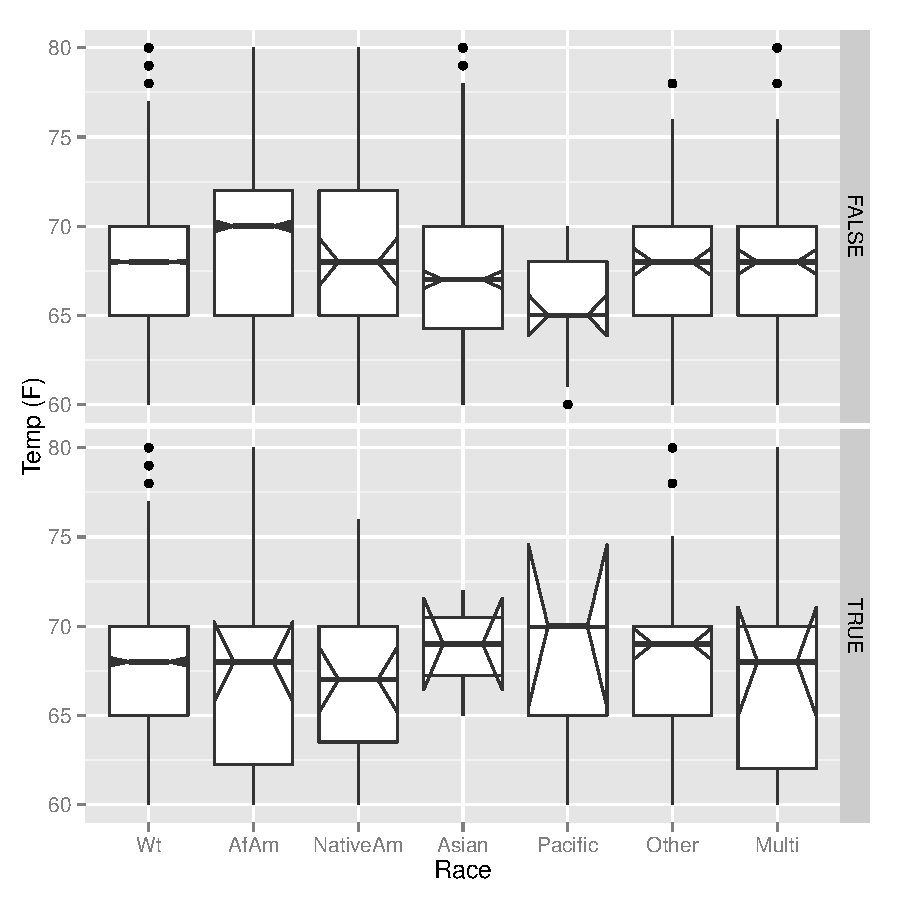
\includegraphics{DraftEdwardsWoods-013}
\end{center}
\end{figure}


\subsection{Differences in Reported Behavior}
  
  \begin{itemize}
    \item Differences in thermostat settings
    \item difference in cooking behavior x
    \item difference in reported AC use

  \end{itemize}
  
  
% latex table generated in R 3.0.1 by xtable 1.7-4 package
% Fri Mar 27 15:58:48 2015
\begin{table}[ht]
\centering
\begin{tabular}{rrrrrrrr}
  \hline
 & Never & ThreeDay & TwoDay & OneDay & FewWeek & OneWeek & LessWeek \\ 
  \hline
FALSEWt &  67 & 452 & 1814 & 3303 & 1825 & 254 & 275 \\ 
  FALSEAfAm &  11 & 156 & 351 & 341 & 448 &  80 &  68 \\ 
  FALSEAsian &   4 &  63 & 111 & 148 &  91 &  13 &  15 \\ 
  FALSEMulti &   2 &  14 &  45 &  40 &  36 &   7 &   2 \\ 
  FALSENativeAm &   0 &   7 &  22 &  27 &  11 &   3 &   3 \\ 
  FALSEOther &   2 &  10 &  25 &  21 &  43 &   3 &   7 \\ 
  FALSEPacific &   0 &   3 &   9 &  10 &  11 &   0 &   3 \\ 
  TRUEAfAm &   1 &   4 &   7 &  13 &   9 &   0 &   0 \\ 
  TRUEAsian &   0 &   0 &   1 &   3 &   2 &   0 &   0 \\ 
  TRUEMulti &   0 &   2 &   1 &  11 &   5 &   2 &   0 \\ 
  TRUENativeAm &   0 &   3 &  12 &  15 &   4 &   2 &   1 \\ 
  TRUEOther &   0 &  20 &  28 &  31 &  14 &   3 &   3 \\ 
  TRUEPacific &   0 &   3 &   0 &   1 &   0 &   0 &   0 \\ 
  TRUEWt &  22 & 208 & 453 & 435 & 226 &  42 &  62 \\ 
   \hline
\end{tabular}
\caption{Weekly Meals Cooked by Race and Ethnicity} 
\label{tab:Cooking}
\end{table}
\begin{figure}
\begin{center}
\caption{Daytime Temp and Race/Ethnicity (Winter)}
\label{fig:TempHomeRace}
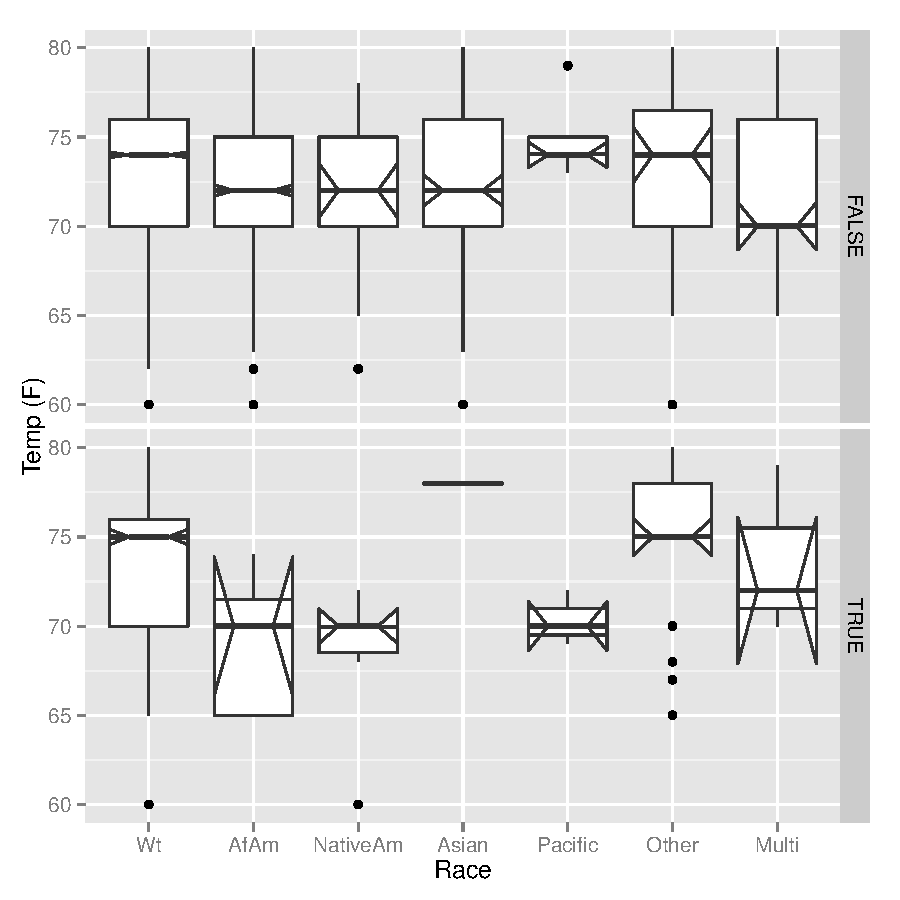
\includegraphics{DraftEdwardsWoods-015}
\end{center}
\end{figure}

\begin{figure}
\begin{center}
\caption{Daytime Temp When Away and Race/Ethnicity (Winter)}
\label{fig:DayAwayRace}
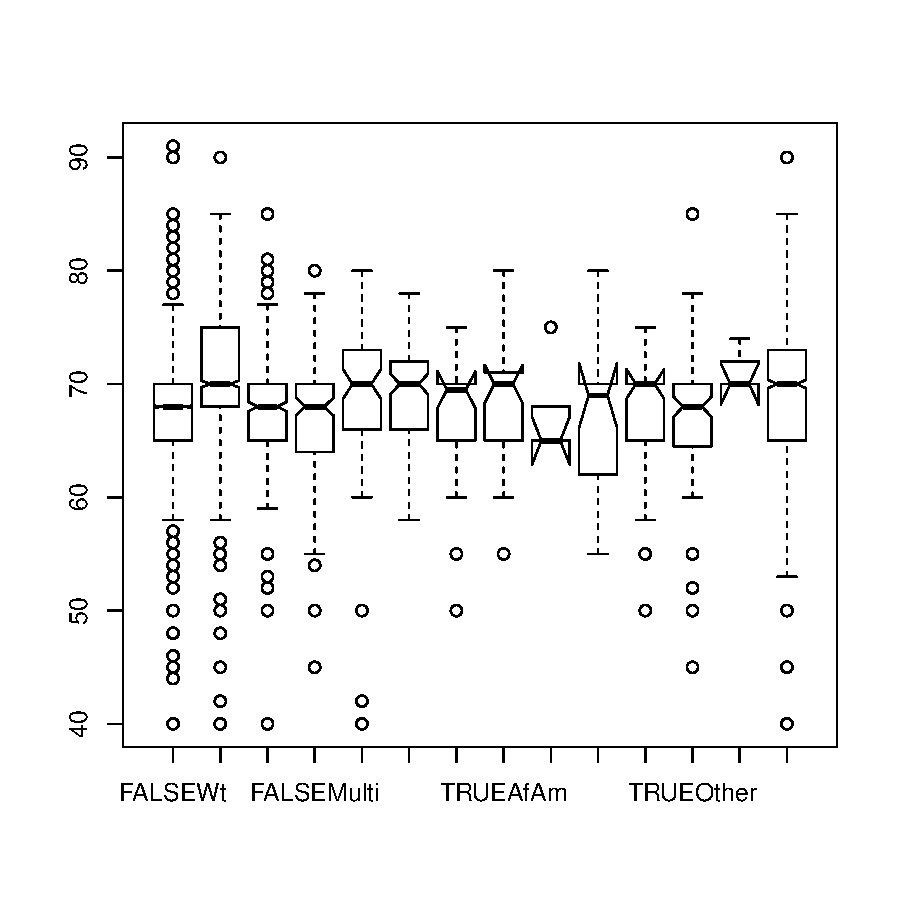
\includegraphics{DraftEdwardsWoods-016}
\end{center}
\end{figure}


\begin{figure}
\begin{center}
\caption{Nighttime Temp and Race/Ethnicity (Winter)}
\label{fig:NightRace}
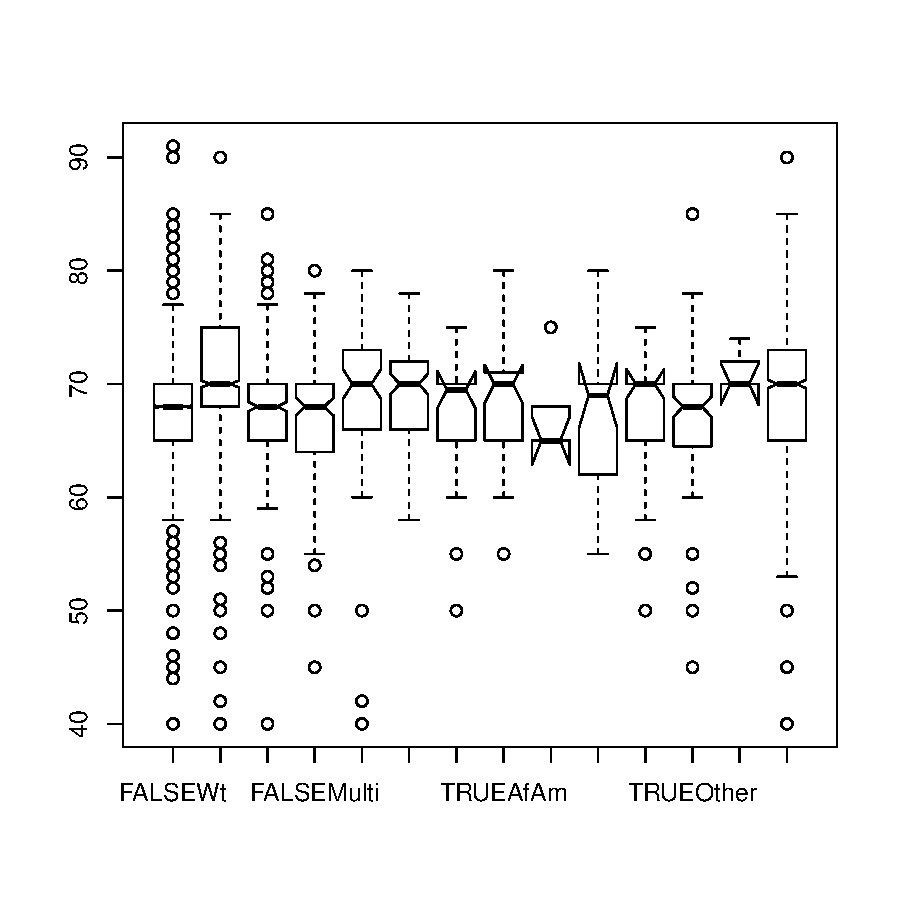
\includegraphics{DraftEdwardsWoods-017}
\end{center}
\end{figure}



\begin{figure}
\begin{center}
\caption{Daytime Temp Home by Race/Ethnicity (Summer)}
\label{fig:HomeRaceS}
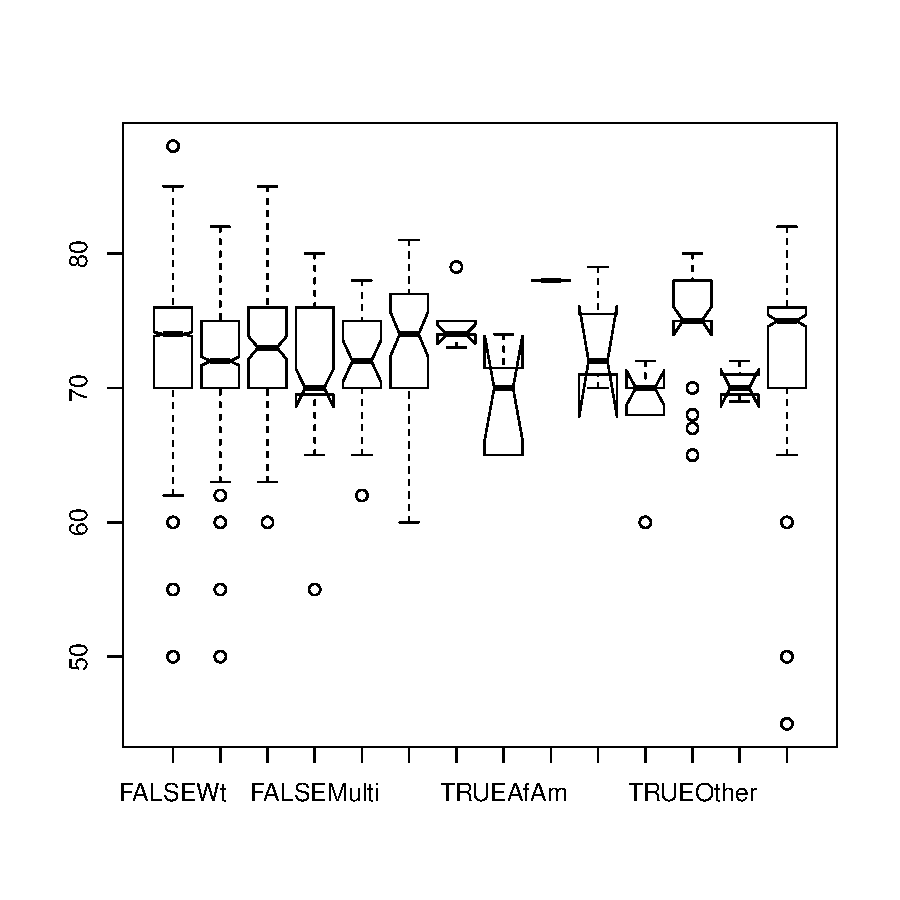
\includegraphics{DraftEdwardsWoods-018}
\end{center}
\end{figure}


\begin{figure}
\begin{center}
\caption{Day Temp Away by Race/Ethnicity (Summer)}
\label{fig:AwayRaceS}
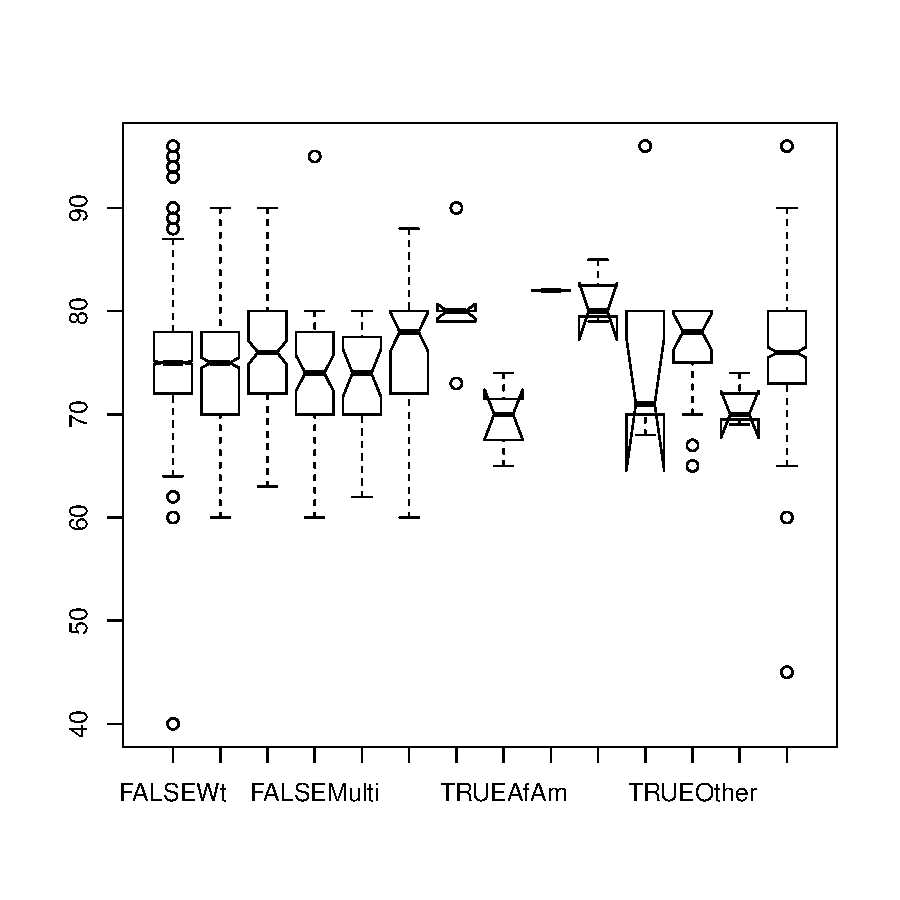
\includegraphics{DraftEdwardsWoods-019}
\end{center}
\end{figure}


\begin{figure}
\begin{center}
\caption{Nighttime Temp and Race/Ethnicity (Summer)}
\label{fig:NightRaceS}
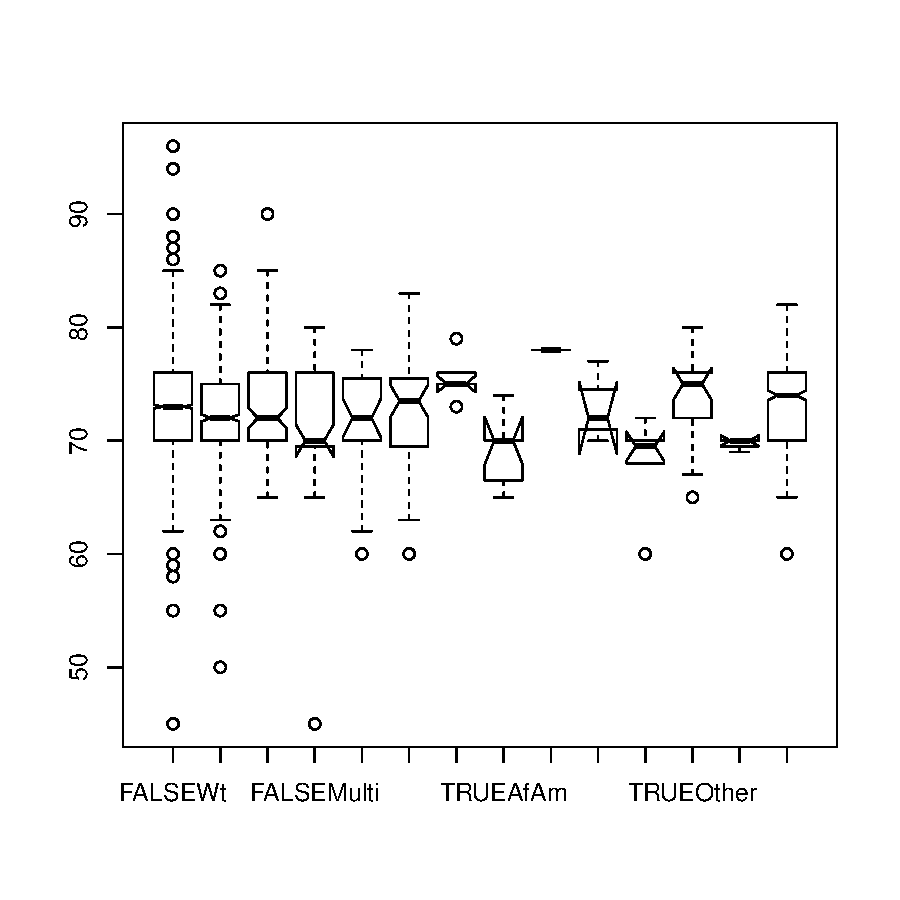
\includegraphics{DraftEdwardsWoods-020}
\end{center}
\end{figure}
  
  \subsection{HUD Complaints as a Measure of Discrimination}\label{sec:WhyHUD}
  
  \begin{itemize}
    \item trouble finding a good statewide index of housing discrimination
    \item the HUD complaint measure
    \item may be endogenous and be indicative of reduced discrimination
  
  \end{itemize}

% latex table generated in R 3.0.1 by xtable 1.7-4 package
% Fri Mar 27 15:58:48 2015
\begin{table}[ht]
\centering
\begin{tabular}{rllr}
  \hline
 & State & Population & Reports (per 100,000) \\ 
  \hline
1 & Alabama & 4,677,464 & 7.50 \\ 
  2 & Alaska & 688,125 & 13.01 \\ 
  3 & Arizona & 6,499,377 & 3.68 \\ 
  4 & Arkansas & 2,867,764 & 9.26 \\ 
  5 & California & 36,580,371 & 3.03 \\ 
  6 & Colorado & 4,935,213 & 1.97 \\ 
  7 & Connecticut & 3,502,932 & 20.50 \\ 
  8 & Delaware & 876,211 & 14.00 \\ 
  9 & District of Columbia & 590,074 & 14.00 \\ 
  10 & Florida & 18,423,878 & 3.93 \\ 
  11 & Georgia & 9,697,838 & 2.06 \\ 
  12 & Hawaii & 1,287,481 & 13.01 \\ 
  13 & Idaho & 1,527,506 & 9.94 \\ 
  14 & Illinois & 12,842,954 & 2.88 \\ 
  15 & Indiana & 6,388,309 & 9.14 \\ 
  16 & Iowa & 2,993,987 & 19.92 \\ 
  17 & Kansas & 2,797,375 & 10.31 \\ 
  18 & Kentucky & 4,287,931 & 7.50 \\ 
  19 & Louisiana & 4,451,513 & 9.26 \\ 
  20 & Maine & 1,319,691 & 20.50 \\ 
  21 & Maryland & 5,658,655 & 14.00 \\ 
  22 & Massachusetts & 6,543,595 & 4.51 \\ 
  23 & Michigan & 10,002,486 & 4.97 \\ 
  24 & Minnesota & 5,230,567 & 19.92 \\ 
  25 & Mississippi & 2,940,212 & 7.50 \\ 
  26 & Missouri & 5,956,335 & 4.99 \\ 
  27 & Montana & 968,035 & 9.94 \\ 
  28 & Nebraska & 1,781,949 & 10.31 \\ 
  29 & Nevada & 2,615,772 & 5.08 \\ 
  30 & New Hampshire & 1,321,872 & 20.50 \\ 
  31 & New Jersey & 8,663,398 & 2.34 \\ 
  32 & New Mexico & 1,986,763 & 5.08 \\ 
  33 & New York & 19,467,789 & 4.60 \\ 
  34 & North Carolina & 9,247,134 & 4.22 \\ 
  35 & North Dakota & 641,421 & 19.92 \\ 
  36 & Ohio & 11,528,072 & 9.14 \\ 
  37 & Oklahoma & 3,644,025 & 9.26 \\ 
  38 & Oregon & 3,782,991 & 13.01 \\ 
  39 & Pennsylvania & 12,566,368 & 1.87 \\ 
  40 & Rhode Island & 1,053,502 & 20.50 \\ 
  41 & South Carolina & 4,503,280 & 4.22 \\ 
  42 & South Dakota & 804,532 & 19.92 \\ 
  43 & Tennessee & 6,240,456 & 2.61 \\ 
  44 & Texas & 24,304,290 & 4.18 \\ 
  45 & Utah & 2,727,343 & 9.94 \\ 
  46 & Vermont & 621,049 & 20.50 \\ 
  47 & Virginia & 7,795,424 & 2.03 \\ 
  48 & Washington & 6,566,073 & 13.01 \\ 
  49 & West Virginia & 1,814,873 & 14.00 \\ 
  50 & Wisconsin & 5,627,610 & 1.81 \\ 
  51 & Wyoming & 532,981 & 9.94 \\ 
   \hline
\end{tabular}
\caption{HUD Complaints per 100,000 Population} 
\label{tab:HUDComplaints}
\end{table}
\section{Conditional Demand Estimation}

  \subsection{Orthodox Results}
  
  \begin{itemize}
    \item Emphasize that we are making better use of race and ethnicity as a control with income than is common.
    \item We are not using the same estimation method as in RECS estimates of end use.  Our model is much simpler and does not use engineering estimates or significant non-linearity.
    \item Major end-uses are included but relatively unsophisticated.
    \item discuss the orthodox results.
  \end{itemize}
  
  
  
Modern conditional demand models of the kind commonly created as part of the process of data collection of large residential appliance and use surveys such as RECS, include a mix of engineering estimates, survey responses and analyst best estimates to produce energy end-use estimates.  For example, survey respondents will give an age range on the furnace they have installed, the square footage of the residence, and some indication of heating set points.  The analyst will assign a likely efficiency for the furnace based on the average of the age ranges and then estimate hours used based on set points, weather, and the reported thermostat settings.  This produces estimates that are closer to a Statistically Adjusted Engineering (SAE) model than what is normally regarded as a conditional demand model outside of the energy community.

Our model is based more on the traditional conditional demand models, and includes terms for electricity use contingent on: the age of the home, which is a proxy for building code requirements and insulation; the weather, in the form of Heating and Cooling degree days with a base temperature of 65F; Meals cooked at home, to indicate energy use related to food preparation; the number and age of refrigerators, a major end-use;  the number of and types of TVs and computers, as a proxy for major plug loads; the existence of a well pump; weather the residence has electric hot water service; the existence of pools and hot tubs as well as if they are electrically heated; the kind of windows installed, as another indication of shell quality; the number of people in the home; and finally the income, race and ethnicity of the residents.  

%Fix latex ref
The parameter estimates of the full model can be found in appendix 
% \ref{OrthResults}
, partial results are shown in table 
% \ref{tab:ParOrthKWH}
.
  
% latex table generated in R 3.0.1 by xtable 1.7-4 package
% Fri Mar 27 15:58:49 2015
\begin{longtable}{rrrrr}
  \hline
 & Estimate & Std. Error & t value & Pr($>$$|$t$|$) \\ 
  \hline
Income & 0.01 & 0.00 & 5.37 & 0.00 \\ 
  Income:EthRaceFALSEAfAm & 0.00 & 0.00 & 1.14 & 0.25 \\ 
  Income:EthRaceFALSEAsian & -0.02 & 0.00 & -7.16 & 0.00 \\ 
  Income:EthRaceFALSEMulti & -0.02 & 0.01 & -2.43 & 0.02 \\ 
  Income:EthRaceFALSENativeAm & 0.01 & 0.01 & 0.95 & 0.34 \\ 
  Income:EthRaceFALSEOther & -0.02 & 0.01 & -2.99 & 0.00 \\ 
  Income:EthRaceFALSEPacific & -0.02 & 0.01 & -1.18 & 0.24 \\ 
  Income:EthRaceTRUEAfAm & -0.01 & 0.02 & -0.73 & 0.47 \\ 
  Income:EthRaceTRUEAsian & -0.04 & 0.05 & -0.80 & 0.42 \\ 
  Income:EthRaceTRUEMulti & -0.03 & 0.02 & -1.37 & 0.17 \\ 
  Income:EthRaceTRUENativeAm & -0.02 & 0.01 & -1.26 & 0.21 \\ 
  Income:EthRaceTRUEOther & -0.03 & 0.01 & -2.63 & 0.01 \\ 
  Income:EthRaceTRUEPacific & -0.01 & 0.04 & -0.32 & 0.75 \\ 
  Income:EthRaceTRUEWt & -0.02 & 0.00 & -6.29 & 0.00 \\ 
  StrTenureOwnSFDetached:TOTSQFT\_EN:HDD65 & 0.00 & 0.00 & 4.10 & 0.00 \\ 
  StrTenureOwnLgApartment:TOTSQFT\_EN:HDD65 & -0.00 & 0.00 & -0.96 & 0.34 \\ 
  StrTenureOwnMobile:TOTSQFT\_EN:HDD65 & 0.00 & 0.00 & 5.98 & 0.00 \\ 
  StrTenureOwnSFAttached:TOTSQFT\_EN:HDD65 & -0.00 & 0.00 & -0.55 & 0.58 \\ 
  StrTenureOwnSmApartment:TOTSQFT\_EN:HDD65 & 0.00 & 0.00 & 0.54 & 0.59 \\ 
  StrTenureRentLgApartment:TOTSQFT\_EN:HDD65 & -0.00 & 0.00 & -4.00 & 0.00 \\ 
  StrTenureRentMobile:TOTSQFT\_EN:HDD65 & 0.00 & 0.00 & 1.76 & 0.08 \\ 
  StrTenureRentSFAttached:TOTSQFT\_EN:HDD65 & 0.00 & 0.00 & 0.60 & 0.55 \\ 
  StrTenureRentSFDetached:TOTSQFT\_EN:HDD65 & 0.00 & 0.00 & 0.55 & 0.58 \\ 
  StrTenureRentSmApartment:TOTSQFT\_EN:HDD65 & -0.00 & 0.00 & -1.86 & 0.06 \\ 
  StrTenureOwnSFDetached:TOTSQFT\_EN:CDD65 & 0.00 & 0.00 & 19.21 & 0.00 \\ 
  StrTenureOwnLgApartment:TOTSQFT\_EN:CDD65 & -0.00 & 0.00 & -0.82 & 0.41 \\ 
  StrTenureOwnMobile:TOTSQFT\_EN:CDD65 & 0.00 & 0.00 & 7.32 & 0.00 \\ 
  StrTenureOwnSFAttached:TOTSQFT\_EN:CDD65 & 0.00 & 0.00 & 5.01 & 0.00 \\ 
  StrTenureOwnSmApartment:TOTSQFT\_EN:CDD65 & 0.00 & 0.00 & 0.40 & 0.69 \\ 
  StrTenureRentLgApartment:TOTSQFT\_EN:CDD65 & 0.00 & 0.00 & 0.39 & 0.69 \\ 
  StrTenureRentMobile:TOTSQFT\_EN:CDD65 & 0.00 & 0.00 & 6.32 & 0.00 \\ 
  StrTenureRentSFAttached:TOTSQFT\_EN:CDD65 & 0.00 & 0.00 & 4.02 & 0.00 \\ 
  StrTenureRentSFDetached:TOTSQFT\_EN:CDD65 & 0.00 & 0.00 & 9.27 & 0.00 \\ 
  StrTenureRentSmApartment:TOTSQFT\_EN:CDD65 & 0.00 & 0.00 & 2.84 & 0.00 \\ 
   \hline
\hline
\caption{Orthodox kWh Model} 
\label{tab:OrthoKWHLimited}
\end{longtable}
The top parameter, Income, shows the estimate for annual kWh per dollar of income for a household headed by a non-Hispanic Caucasian.  The remaining income related variables show the deviations from this case for Hispanic headed households, labeled TRUE in the table, and by the other self reported races.  Note that in all cases, with the exception of non-Hispanic Native Americans, the parameter estimates show less electricity used than non-Hispanic Caucasian households.  Only a few of these differences are statistically significant, non-Hispanic Asian and multi-ethnic households, as well as Hispanic Caucasian households and households that reported some other race.

The remaining items shown in the table show the electricity use per square foot for each of the structure types, e.g., Single Family Detached, and tenure, i.e., Rent or Own, per annual heating and cooling degree days.  Aside from the negative and significant estimate for the heating load in large Rented apartments, the results are unremarkable. 

\subsection{Endogenizing Structure and Other Variables}\label{sec:SingleEq}

Treating structure type and square footage as endogenous is our first step in estimating conditional demand for many end uses treating the choice of things like, EnergyStar appliances, refrigerator size and design.  The current standard, treating these as exogenous drivers of energy use biases or estimates of energy use in unknown ways.

Focusing on tenure, i.e., the decision to own or rent, structure and square footage decisions allows us to see if other housing market institutions are driving energy use differently depending on ethnicity.  At this early stage of research we are focusing only on these major drivers but we can expand the analysis to other choices including clothes washing, hot water service and other large energy drivers.

As stated in section \ref{sec:WhyHUD}, using HUD complaints as a measure of housing market discrimination based on race and ethnicity is less than optimal measure, but at this early stage is an adequate measure to determine the scale of the effect.  


Table 
% \ref{tab:OrthoSQFTLimited} 
shows only the discrimination related results for our model of square footage.  Full results can be seen in appendix 
% \ref{OrthResults}
.   Note that the square footage model includes structure type and tenure as an exogenous variable.  This model of square footage will be included later as part of a system estimation of electricity use.   

The key discrimination variable, reporttot, is the count of complaints received by HUD per 100,000 people in the state where the household is located. We interacted this variable with race and ethnicity to allow for different effects  groups but we do not allow the discrimination to vary by state. Note that the effects of HUD reports on square footage are rarely significant, only strongly significant for Hispanic Caucasian households.  In this case incidences of HUD complaints per 100,000 of state population results in a reduction in the square footage for Caucasian Hispanics by 22.73 square feet.


% \begin{itemize}
%   \item explain the logic behind the making both sqft and structure tenure endogenous.
%   \item primarily that sqft may be related to quality of houseing, newer structures
% \end{itemize}



While the impact of housing market discrimination has some effect on the size of residences, the effects on the ownership and structure type decision is expected to be more dramatic.  Housing market discrimination can be expected to push some people away from owned property and into the rental market, which is rife with split incentives for conservation and energy efficiency investments.  

Discrimination can also be a force pushing some households into structure types, where even when owned, that have significant split incentives for energy efficiency investments.  Take, for example, small and large apartment buildings.  While the householder may have control over some appliances, the building shell and some of the heating and cooling equipment decisions are made by others.  

Our model of structure type and tenure includes categories for both owned and rented: Large Apartments, Small Apartments, Mobile Homes, Single Family Detached, and Single Family Attached.  We explain the joint tenure and structure type with: the square footage of the structure, if the household receives rental assistance, Income, number of people in the household, education level of the head of household, the HUD reports per 100,000 in that state and whether the household is in a rural or urban location.  As in the square footage model, HUD reports are interacted with the race and ethnicity variables to allow for separate discrimination effects for each.


All parameter estimates for the models are statistically significant at the 1\% level and are displayed in appendix 
% \ref{OrthResults}. 


%Fix the Latex part of this.
Since all the parameters are statistically significant it is easier to show the effects of our measure of housing market discrimination on the probability of each structure and tenure choice for the race and ethnicity combinations.  The HUD reports run from 1.81249 complaints per 100,000 to 20.496 complaints per 100,000.  Figure 
% \ref{fig:HUDOnChoice} 
shows the reaction to HUD complaints over the 1 to 21 complaint range.


% 
% \begin{figure}
% \begin{center}\label{fig:HUDOnChoice}
% 
% <<echo=false,fig=TRUE>>=
% # Need to figure this figure out.  It may be very complex
% 
% @
% \end{center}
% \end{figure}

***Lots of explanation goes here***




  \subsection{System Estimation}

The single equation results discussed in section \ref{sec:SingleEq} show strong promise for endogenizing some of the decisions made about structure and equipment within the conditional demand model as well as the potential importance of housing market discrimination in structure choice.  In this section we treat square footage, tenure and structure type as endogenous and estimate estimate the electricity, structure/tenure, and square footage model as a system.

It is unclear how this can be accomplished in a full information, so we chose a two-state least squares technique estimating first the square footage model, then using forecasted values to estimate tenure and structure type model.  Forecasts from that model were used to resestimate and produce a new round of forecasts for the square footage model.  Both the forecasts of the structure tenure model and square footage model were then used to estimate the conditional demand model.

This should produce consistent results but the variance of the parameter estimates are biased.  It is unclear how to make the usual corrections to the variance of the parameter estimates given that the structure and tenure model is estimated as a multinomial logit.  The best alternative is to bootstrap the system.  There are a few caveats.

First, the bootstrap sampling is stratified so that all parameter estimates in all models can be estimated.  This is particularly important in the structure and tenure model.  We had to ensure enough observations of the rare endogenouse cells, rented mobile homes being the most restricted, and exogenous variables, e.g., Hispanic Pacific Islanders.  This was accomplished by simple rejection sampling rather than assigning different probabilities of selection to each of the cells.

Second, we did not censor non-positive square footage forecasts.  The square footage model is weaker than expected and it was quite possible to have negative forecasts.  Alternative models, such as Tobit, would not be effective, but we are considering transformations of square footage as we move forward.  

Finally, only 400 bootstrap replicates were evaluated.  This is usually enough to produce adequate estimates of the standard deviations of the parameter estimates in the electricity model but insufficient for BCa, percentile, or even basic bootstrap confidence intervals. 

% \begin{itemize}
%   \item results are bootstrapped 400 times for standard deviation estimates.  More can be done.
%   \item probablities of structure type rather than forecast were used.
%   \item no censoring for square footage less than zero.
%   \item boot strap samples were restricted to samples that allowed for all parameters to be estimated.
% \end{itemize}


